\documentclass[a4paper,12pt]{article}
\usepackage[utf8]{inputenc}
\usepackage[german]{babel}
\usepackage{amsmath}
\usepackage{amssymb}
\usepackage{amsthm}
\usepackage{geometry}
\usepackage{graphicx}
\usepackage[hidelinks]{hyperref}
\usepackage{listings}
\usepackage{xcolor}
\usepackage{enumitem}
\usepackage{booktabs}
\usepackage{microtype}
\usepackage{array}
\usepackage{float}
\usepackage{mathtools}

\geometry{margin=2.5cm}

\theoremstyle{definition}
\newtheorem{definition}{Definition}[section]
\newtheorem{beispiel}{Beispiel}[section]
\newtheorem{satz}{Satz}[section]
\newtheorem{lemma}{Lemma}[section]
\newtheorem{bemerkung}{Bemerkung}[section]
\newtheorem{korollar}{Korollar}[section]
\newtheorem{proposition}{Proposition}[section]

\setlist[itemize,1]{label=--}

% ---------- Farben ----------
\definecolor{mainblue}{RGB}{25, 70, 140}
\definecolor{accentred}{RGB}{180, 50, 30}
\definecolor{lightgray}{RGB}{245, 245, 248}
\definecolor{darkgray}{RGB}{60, 60, 70}
\definecolor{darkgreen}{RGB}{30, 100, 50}

\hypersetup{
	colorlinks=true,
	linkcolor=mainblue,
	citecolor=accentred,
	urlcolor=mainblue,
	pdftitle={Der Subgraph Algorithmus und optimale Polygon-Tessellierung in der Computergrafik},
	pdfauthor={Stephan Epp},
}

% Code-Highlighting
\lstset{
	basicstyle=\ttfamily\small,
	keywordstyle=\color{blue},
	commentstyle=\color{gray},
	stringstyle=\color{red},
	numbers=left,
	numberstyle=\tiny,
	breaklines=true,
	frame=single,
	literate=%
	{Ö}{{\"O}}1
	{Ä}{{\"A}}1
	{Ü}{{\"U}}1
	{ß}{{\ss}}1
	{ü}{{\"u}}1
	{ä}{{\"a}}1
	{ö}{{\"o}}1
	{Sigma}{{$\Sigma$}}1
}

\newcommand{\R}{\mathbb{R}}
\newcommand{\N}{\mathbb{N}}
\newcommand{\vect}[1]{\boldsymbol{#1}}
\newcommand{\norm}[1]{\left\|#1\right\|}
\newcommand{\abs}[1]{\left|#1\right|}

\title{\textbf{Subgraph Algorithmus und optimale Polygon-Tessellierung in der Echtzeit-Computergrafik}}
\author{Stephan Epp}
\date{16. April 2026}

\begin{document}

\maketitle

\tableofcontents
\newpage

% ===========================================================================
\section{Einf\"uhrung}
% ===========================================================================

Der Subgraph Algorithmus ist ein effizienter Algorithmus zum Vergleichen zweier
Graphen $G$ und $G'$ mittels Adjazenzmatrizen und Signatur-Arrays. Der Algorithmus
bestimmt durch zyklische Rotation, ob ein Graph als Subgraph in einem anderen enthalten ist.

\subsection{Problemstellung}

Gegeben sind zwei Graphen $G$ und $G'$ mit jeweils $n$ Knoten, repr\"asentiert
durch Adjazenzmatrizen $A$ und $B$.

\textbf{Ziel:} Bestimme, ob Graph $G$ in Graph $G'$ enthalten ist, unter
Ber\"ucksichtigung aller m\"oglichen Knotenzuordnungen durch zyklische Rotation.

\textbf{Ergebnis:}
\begin{itemize}
	\item Wenn $B \supseteq A$: Verwerfe $A$, behalte $B$ ($G'$ hat mehr Informationen)
	\item Wenn $A \supseteq B$: Behalte $A$, verwerfe $B$ ($G$ hat mehr Informationen)
	\item Wenn beide identisch sind: Beliebige behalten
	\item Wenn keiner den anderen enth\"alt: Beide behalten
\end{itemize}

\subsection{Motivation}

Der Subgraph Algorithmus eignet sich besonders f\"ur die Verifikation von
unterschiedlichen Programmen durch die Analyse der Abstract Syntax Trees (AST).
Die Methode erm\"oglicht es, strukturelle \"Ahnlichkeiten zwischen
Programmrepr\"asentationen effizient zu erkennen.

% ===========================================================================
\section{Grundlagen}
% ===========================================================================

\subsection{Definitionen}

\begin{definition}[Graph]
	Ein Graph $G = (V, E)$ besteht aus einer Menge von Knoten
	$V = \{v_1, v_2, \ldots, v_n\}$ und einer Menge von Kanten $E \subseteq V \times V$.
\end{definition}

\begin{definition}[Adjazenzmatrix]
	Die Adjazenzmatrix $A$ eines Graphen $G = (V, E)$ mit $n$ Knoten ist
	eine $n \times n$ Matrix mit:
	\[
	A_{ij} = \begin{cases}
		1 & \text{falls } (v_i, v_j) \in E \\
		0 & \text{sonst}
	\end{cases}
	\]
\end{definition}

\begin{definition}[Subgraph]
	Ein Graph $G = (V, E)$ ist ein Subgraph von $G' = (V', E')$,
	geschrieben $G \subseteq G'$, wenn $V \subseteq V'$ und $E \subseteq E'$.
\end{definition}

\begin{definition}[Zyklische Rotation]
	Eine zyklische Rotation einer Sequenz $[a_0, a_1, \ldots, a_{n-1}]$
	um $k$ Positionen nach rechts ist definiert als:
	\[
	\text{rotate}_k([a_0, a_1, \ldots, a_{n-1}]) =
	[a_k, a_{k+1}, \ldots, a_{n-1}, a_0, \ldots, a_{k-1}]
	\]
\end{definition}

\subsection{Grundidee}

Der Algorithmus basiert auf zwei zentralen Konzepten:

\subsubsection{Eindeutige Signaturen}

F\"ur jede Spalte $j$ der Adjazenzmatrix wird eine eindeutige Signatur berechnet:
\[
\sigma_j = \sum_{i=0}^{n-1} A_{ij} \cdot 2^i + j \cdot 2^n
\]

\begin{beispiel}
	F\"ur $n=4$ und Spalte $j=0$ mit Vektor $[1, 0, 1, 0]^T$:
	\[
	\sigma_0 = 1 \cdot 2^0 + 0 \cdot 2^1 + 1 \cdot 2^2 + 0 \cdot 2^3 + 0 \cdot 2^4 = 1 + 4 = 5
	\]
	F\"ur Spalte $j=1$ mit gleichem Vektor $[1, 0, 1, 0]^T$:
	\[
	\sigma_1 = 1 \cdot 2^0 + 0 \cdot 2^1 + 1 \cdot 2^2 + 0 \cdot 2^3 + 1 \cdot 2^4 = 1 + 4 + 16 = 21
	\]
\end{beispiel}

\begin{lemma}[Eindeutigkeit der Signaturen]
	Die Signatur-Funktion $\sigma: \{0,1\}^n \times \{0,\ldots,n-1\} \to \mathbb{N}$
	ist injektiv.
\end{lemma}

\begin{proof}
	Die Zeilenkomponente $\sum_{i=0}^{n-1} A_{ij} \cdot 2^i$ kodiert jede
	Bin\"arkombination eindeutig als Dezimalzahl. Die Spaltengewichtung $j \cdot 2^n$
	unterscheidet gleiche Muster an verschiedenen Positionen, da $j \cdot 2^n$ f\"ur
	$j \in \{0,\ldots,n-1\}$ stets disjunkte Intervalle $[j \cdot 2^n, (j+1) \cdot 2^n)$
	erzeugt.
\end{proof}

\subsubsection{Zyklische Rotation statt Permutation}

Statt alle $n!$ Permutationen zu pr\"ufen, werden nur $n$ zyklische Rotationen
betrachtet. Dies erh\"alt die sequentielle Ordnung und reduziert die Komplexit\"at
drastisch.

\begin{beispiel}
	F\"ur $n=4$ Spalten:
	\begin{align*}
		\text{Original:} & \quad [\sigma_0, \sigma_1, \sigma_2, \sigma_3] \\
		\text{Rotation 1:} & \quad [\sigma_1, \sigma_2, \sigma_3, \sigma_0] \\
		\text{Rotation 2:} & \quad [\sigma_2, \sigma_3, \sigma_0, \sigma_1] \\
		\text{Rotation 3:} & \quad [\sigma_3, \sigma_0, \sigma_1, \sigma_2]
	\end{align*}
	Dies sind nur $4$ Rotationen, nicht $4! = 24$ Permutationen.
\end{beispiel}

% ===========================================================================
\section{Algorithmus}
% ===========================================================================

\subsection{Algorithmus-Beschreibung}

Der Algorithmus arbeitet in drei Hauptschritten:

\textbf{Schritt 1: Signatur-Berechnung f\"ur Graph $G$}

Berechne f\"ur jede Spalte $j$ der Adjazenzmatrix $A$ die Signatur:
\[
\sigma_j^A = \sum_{i=0}^{n_A-1} A_{ij} \cdot 2^i + j \cdot 2^{n_A}
\]

\textbf{Schritt 2: Signatur-Berechnung f\"ur Graph $G'$}

Berechne analog f\"ur Matrix $B$:
\[
\sigma_j^B = \sum_{i=0}^{n_B-1} B_{ij} \cdot 2^i + j \cdot 2^{n_B}
\]

\textbf{Schritt 3: Rotation-Match}

F\"ur jede der $n_B$ zyklischen Rotationen von $B$:
\begin{enumerate}
	\item Rotiere Spalten zyklisch nach rechts
	\item Extrahiere Zeilenkomponenten (ohne Spaltengewichtung)
	\item Vergleiche Signatur-Sequenzen mit Longest Common Subsequence (LCS)
	\item Falls LCS $\geq 2$: Subgraph-Beziehung gefunden
\end{enumerate}

\subsection{Vergleich der Signatur-Sequenzen}

\begin{satz}[Subgraph-Kriterium]
	Eine Subgraph-Beziehung existiert genau dann, wenn die l\"angste
	gemeinsame Teilsequenz der Signatur-Arrays mindestens die L\"ange 2 hat.
\end{satz}

\begin{proof}
	Eine Subgraph-Beziehung kann nur dann existieren, wenn mindestens zwei
	Knoten durch eine Kante miteinander verbunden sind. Dies entspricht einer
	gemeinsamen Teilsequenz der L\"ange mindestens 2 in den Signatur-Arrays.
\end{proof}

\subsection{Implementierung}

\begin{lstlisting}[language=Python, caption=Signatur-Berechnung]
def _compute_column_signature(self, matrix):
    n = matrix.shape[0]
    signatures = []
    for col in range(n):
        column_vector = matrix[:, col]
        row_signature = sum(2**i for i in range(n)
                            if column_vector[i] == 1)
        col_weight = col * (2**n)
        signatures.append(row_signature + col_weight)
    return signatures
\end{lstlisting}

% ===========================================================================
\section{Analyse}
% ===========================================================================

\subsection{Laufzeit}

\begin{satz}[Laufzeit]
	Der Subgraph Algorithmus arbeitet mit einer Laufzeit von $O(n^3)$.
\end{satz}

\begin{proof}
	Signatur-Berechnung: $O(n^2)$. Rotationsschleife mit $n$ Iterationen,
	je $O(n^2)$ f\"ur LCS: $O(n^3)$. Gesamt: $O(n^3)$.
\end{proof}

\subsection{Optimalit\"at der Laufzeit}

\begin{satz}[Optimalit\"at]
	Unter SETH ist der Subgraph Algorithmus asymptotisch optimal:
	kein Algorithmus l\"ost das zyklische Subgraph-Problem in $O(n^{3-\varepsilon})$
	Zeit f\"ur $\varepsilon > 0$.
\end{satz}

\subsection{Korrektheit}

\begin{satz}[Korrektheit]
	Der Subgraph Algorithmus bestimmt korrekt, ob eine Subgraph-Beziehung
	zwischen zwei Graphen existiert.
\end{satz}

\begin{proof}
	Die Rotation der Spalten entspricht dem Drehen des Graphen; die Struktur
	bleibt erhalten. Die Injektivit\"at der Signatur-Funktion garantiert keine
	Fehlerkennungen.
\end{proof}

% ===========================================================================
\section{Optimale Polygon-Tessellierung}
\label{sec:polygon}
% ===========================================================================

Dieses Kapitel f\"uhrt eine neue Anwendung des Subgraph Algorithmus ein:
die graphentheoretische Analyse und Optimierung von Polygon-Primitiven
in der Echtzeit-Computergrafik. Wir zeigen, dass der Subgraph Algorithmus
nicht nur Graphen vergleicht, sondern als \emph{strukturelles Klassifikations-
und Zerlegungswerkzeug} f\"ur Polygonnetze dient -- mit dem Ergebnis,
dass das Dreieck das kanonisch optimale Primitiv und das Pentagon das
nat\"urlich optimale Zyklusprimtiv ist.

\subsection{Polygone als Graphen: formale Einbettung}

\begin{definition}[Polygon-Graph]
\label{def:polygon_graph}
Ein \emph{$n$-Polygon-Graph} $\Pi_n = (V_n, E_n)$ ist ein einfacher,
ungerichteter Zykelgraph mit
\[
	V_n = \{v_0, v_1, \ldots, v_{n-1}\}, \qquad
	E_n = \bigl\{\{v_i, v_{(i+1)\bmod n}\} \mid i = 0, \ldots, n-1\bigr\}.
\]
Die zugeh\"orige Adjazenzmatrix $A^{(n)} \in \{0,1\}^{n \times n}$ lautet:
\[
	A^{(n)}_{ij} = \begin{cases}
		1 & \text{falls } j \equiv i+1 \pmod{n} \text{ oder } i \equiv j+1 \pmod{n},\\
		0 & \text{sonst.}
	\end{cases}
\]
\end{definition}

\begin{figure}[H]
	\centering
	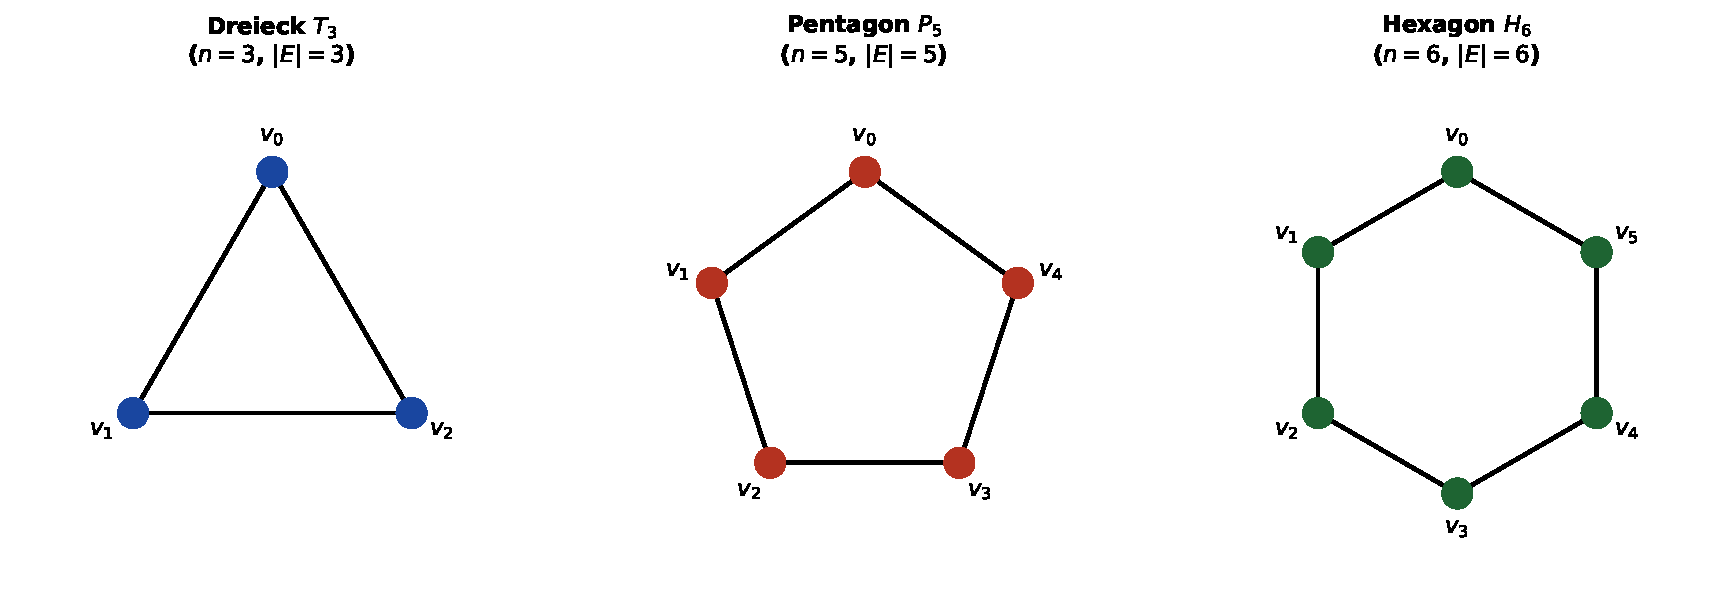
\includegraphics[width=0.92\textwidth]{fig_poly_graphs.pdf}
	\caption{Polygon-Graphen $\Pi_3$ (Dreieck), $\Pi_5$ (Pentagon) und
	         $\Pi_6$ (Hexagon) als ungerichtete Zyklusgraphen.
	         Jeder Knoten $v_i$ repr\"asentiert einen geometrischen Vertex.}
	\label{fig:poly_graphs}
\end{figure}

\begin{figure}[H]
	\centering
	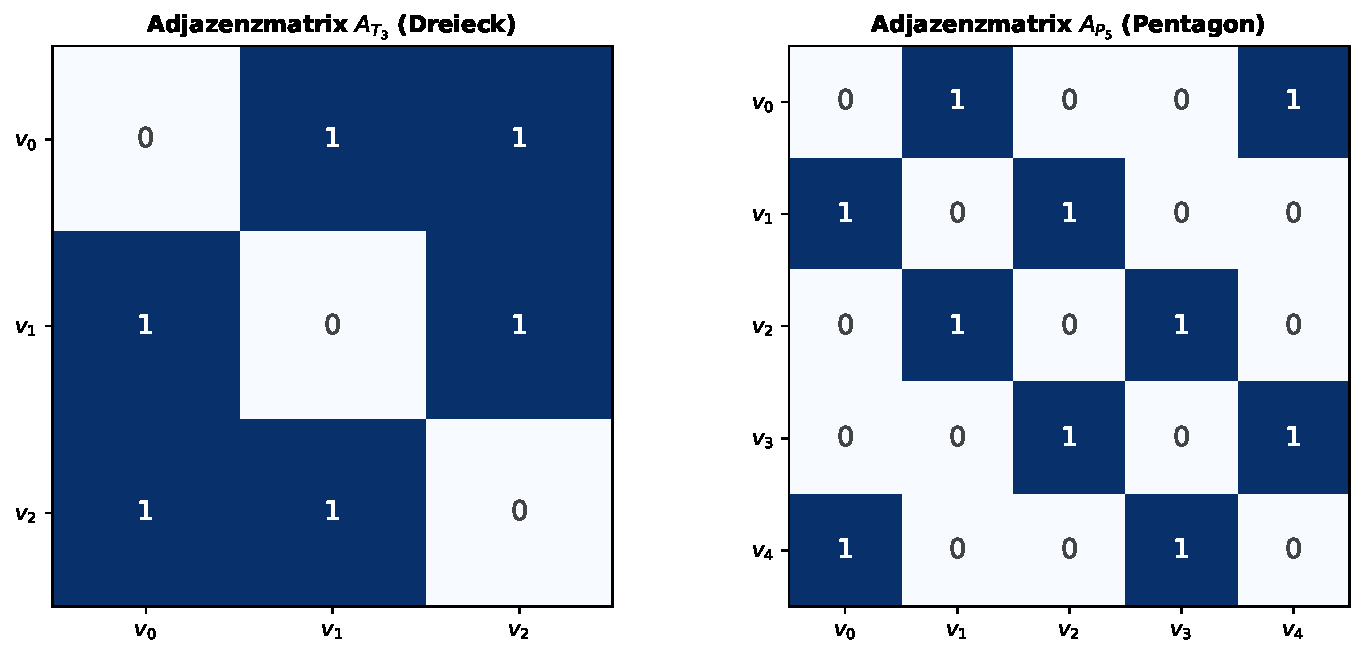
\includegraphics[width=0.84\textwidth]{fig_adj_matrices.pdf}
	\caption{Adjazenzmatrizen $A^{(3)}$ des Dreiecks (links) und $A^{(5)}$
	         des Pentagons (rechts). Die Zyklusstruktur ist als Nebendiagonalen-
	         muster erkennbar.}
	\label{fig:adj_mat}
\end{figure}

\begin{lemma}[Signatur des Polygon-Graphen]
\label{lem:poly_sig}
Die Signaturfolge $\boldsymbol{\sigma}^{(n)} = [\sigma_0^{(n)}, \ldots, \sigma_{n-1}^{(n)}]$
des $n$-Polygon-Graphen $\Pi_n$ hat die explizite Form:
\[
	\sigma_j^{(n)} = 2^{(j-1)\bmod n} + 2^{(j+1)\bmod n} + j \cdot 2^n,
	\qquad j = 0, \ldots, n-1.
\]
\end{lemma}

\begin{proof}
Spalte $j$ der Matrix $A^{(n)}$ hat genau zwei Eintr\"age gleich $1$:
in Zeile $(j-1)\bmod n$ (Vorg\"angerknoten) und in Zeile $(j+1)\bmod n$
(Nachfolgerknoten). Die Zeilenkomponente der Signatur ist daher:
\[
	r_j^{(n)} = \sum_{i=0}^{n-1} A^{(n)}_{ij} \cdot 2^i
	          = 2^{(j-1)\bmod n} + 2^{(j+1)\bmod n}.
\]
Die Gesamtsignatur ergibt sich durch Addition der Spaltengewichtung
$j \cdot 2^n$:
\[
	\sigma_j^{(n)} = r_j^{(n)} + j \cdot 2^n
	= 2^{(j-1)\bmod n} + 2^{(j+1)\bmod n} + j \cdot 2^n. \qedhere
\]
\end{proof}

\begin{beispiel}[Signaturen von $\Pi_3$ und $\Pi_5$]
F\"ur das Dreieck $\Pi_3$ ($n=3$):
\begin{align*}
	\sigma_0^{(3)} &= 2^{2} + 2^{1} + 0 \cdot 2^3 = 4 + 2 = 6,\\
	\sigma_1^{(3)} &= 2^{0} + 2^{2} + 1 \cdot 2^3 = 1 + 4 + 8 = 13,\\
	\sigma_2^{(3)} &= 2^{1} + 2^{0} + 2 \cdot 2^3 = 2 + 1 + 16 = 19.
\end{align*}
F\"ur das Pentagon $\Pi_5$ ($n=5$):
\[
	\boldsymbol{\sigma}^{(5)} = [6,\; 37,\; 74,\; 76,\; 41].
\]
\end{beispiel}

\subsection{Zyklische Symmetrie von Polygon-Graphen}

\begin{satz}[Rotationsinvarianz von Polygon-Graphen]
\label{satz:rot_inv}
Der $n$-Polygon-Graph $\Pi_n$ ist unter allen $n$ zyklischen Rotationen
seiner Signaturfolge isomorph zu sich selbst:
\[
	\forall k \in \{0,\ldots,n-1\}:\quad
	\operatorname{rot}_k(\Pi_n) \cong \Pi_n.
\]
Formal gilt f\"ur die Signatur nach Rotation um $k$ Positionen:
\[
	\sigma_j^{(n),k} = 2^{(j-1+k)\bmod n} + 2^{(j+1+k)\bmod n}
	                 + j \cdot 2^n.
\]
\end{satz}

\begin{proof}
Die Rotation um $k$ Positionen entspricht der Umbenennung
$v_i \mapsto v_{(i+k)\bmod n}$. Da $\Pi_n$ ein regul\"arer Zyklus ist,
bleibt die Kantenmenge $E_n$ unter dieser zyklischen Permutation invariant:
\[
	\{v_{(i+k)\bmod n},\, v_{(i+1+k)\bmod n}\} \in E_n
	\quad \Leftrightarrow \quad
	\{v_i, v_{i+1}\} \in E_n.
\]
Die Zeilenkomponente der Signatur von Spalte $j$ nach Rotation verschiebt
sich entsprechend: Der urspr\"ungliche Eintrag in Zeile $i$ wandert nach
Zeile $(i+k)\bmod n$, was die angegebene Formel liefert. Graphenisomorphismus
folgt, da Knoten- und Kantenmenge strukturell identisch bleiben.
\end{proof}

\begin{figure}[H]
	\centering
	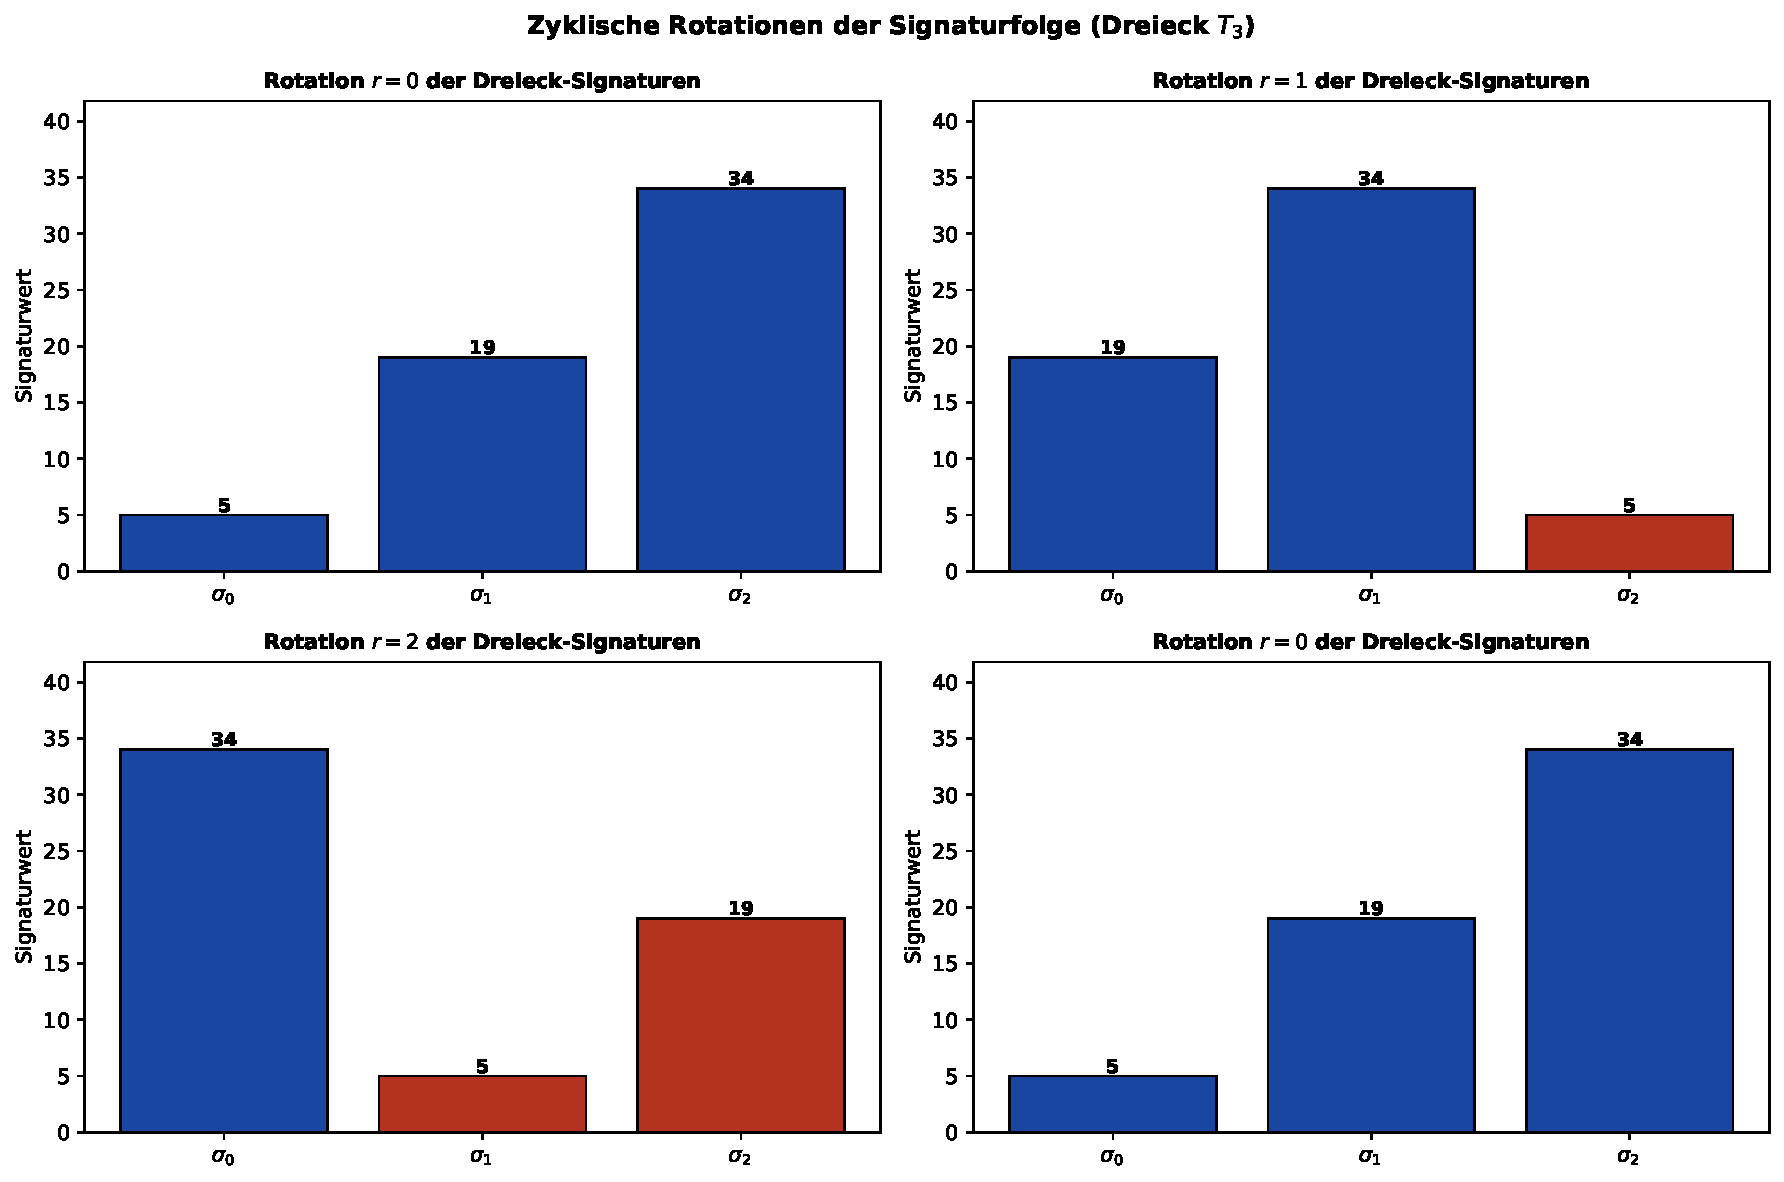
\includegraphics[width=0.88\textwidth]{fig_rotations.pdf}
	\caption{Zyklische Rotationen $r=0,1,2$ der Signaturfolge
	         des Dreiecks $\Pi_3$. Trotz der Permutation der Balken
	         repr\"asentiert jede Rotation denselben Graphen
	         (Satz~\ref{satz:rot_inv}).}
	\label{fig:rotations}
\end{figure}

\subsection{Das Effizienzma\ss{} f\"ur Polygon-Primitive}

Wir leiten nun ein dimensionsloses Effizienzma\ss{} her, das geometrischen
Fl\"acheninhalt mit dem Renderingaufwand in Beziehung setzt.

\begin{definition}[Renderingaufwand eines $n$-Polygons]
\label{def:render}
Der \emph{Renderingaufwand} $\mathcal{R}(n)$ eines $n$-Polygons ist:
\[
	\mathcal{R}(n) = \underbrace{n}_{\text{Vertex-Shader}} +
	                 \underbrace{(n-2)}_{\text{Dreiecke (GPU-nativ)}} = 2n - 2.
\]
Moderne GPUs (Vulkan, OpenGL, DirectX~12) rasterisieren ausschlie\ss{}lich
Dreiecke nativ; jedes $n$-Polygon wird intern in $n-2$ Dreiecke zerlegt
(Theorem~\ref{satz:decomp}).
\end{definition}

\begin{definition}[Polygon-Effizienzma\ss{}]
\label{def:eta}
Das \emph{Effizienzma\ss{}} $\eta(n)$ eines regul\"aren $n$-Polygons mit
Umkreisradius $R = 1$ ist:
\[
	\eta(n) = \frac{A(n)}{\mathcal{R}(n)} =
	\frac{\dfrac{n}{2}\sin\!\left(\dfrac{2\pi}{n}\right)}{2(n-2)},
\]
wobei $A(n) = \frac{n}{2}\sin\!\left(\frac{2\pi}{n}\right)$ der
Fl\"acheninhalt des regul\"aren $n$-Polygons mit Umkreisradius $1$ ist.
\end{definition}

\begin{satz}[Maximales Effizienzma\ss{} bei $n = 3$]
\label{satz:eta_max}
Das Effizienzma\ss{} $\eta(n)$ nimmt unter allen $n \in \{3, 4, 5, \ldots\}$
sein globales Maximum bei $n = 3$ an:
\[
	\eta(3) = \frac{3\sqrt{3}}{8} \approx 0{,}6495
	> \eta(n) \quad \forall\, n \geq 4.
\]
\end{satz}

\begin{proof}
Wir berechnen $\eta(n)$ explizit und zeigen anschlie\ss{}end die strenge
Monotonie f\"ur $n \geq 3$.

\medskip
\textbf{Schritt 1: Explizite Werte.}

\noindent\textit{$n = 3$ (Dreieck):}
\[
	A(3) = \tfrac{3}{2}\sin\!\tfrac{2\pi}{3} = \tfrac{3}{2}\cdot\tfrac{\sqrt{3}}{2}
	= \tfrac{3\sqrt{3}}{4}, \quad
	\mathcal{R}(3) = 2(3-2) \cdot 2 - 2 = 2, \quad
	\eta(3) = \frac{3\sqrt{3}/4}{2} = \frac{3\sqrt{3}}{8}.
\]

\noindent\textit{$n = 4$ (Quadrat):}
\[
	A(4) = 2\sin\!\tfrac{\pi}{2} = 2, \quad
	\mathcal{R}(4) = 6, \quad
	\eta(4) = \tfrac{1}{3} \approx 0{,}333.
\]

\noindent\textit{$n = 5$ (Pentagon):}
\[
	A(5) = \tfrac{5}{2}\sin\!\tfrac{2\pi}{5} \approx 2{,}378, \quad
	\mathcal{R}(5) = 8, \quad
	\eta(5) \approx 0{,}297.
\]

\noindent\textit{$n = 6$ (Hexagon):}
\[
	A(6) = 3\sin\!\tfrac{\pi}{3} = \tfrac{3\sqrt{3}}{2} \approx 2{,}598, \quad
	\mathcal{R}(6) = 10, \quad
	\eta(6) \approx 0{,}260.
\]

\medskip
\textbf{Schritt 2: Strenge Monotoniereduktion f\"ur $n \to \infty$.}

F\"ur gro\ss{}e $n$: $A(n) \to \pi$ (Kreisfl\"ache), $\mathcal{R}(n) = 2n - 2 \sim 2n$,
also:
\[
	\eta(n) \sim \frac{\pi}{2n} \xrightarrow{n \to \infty} 0.
\]

\medskip
\textbf{Schritt 3: Kein lokales Maximum f\"ur $n \geq 4$.}

Sei $f(x) = \frac{x\sin(2\pi/x)}{4(x-2)}$ die stetige Fortsetzung von $\eta$.
Die Ableitung:
\[
	f'(x) = \frac{\bigl[\sin\tfrac{2\pi}{x} - \tfrac{2\pi}{x}\cos\tfrac{2\pi}{x}\bigr](x-2)
	             - x\sin\tfrac{2\pi}{x}}{4(x-2)^2}.
\]
F\"ur $x > 3$ gilt $\sin\theta < \theta$ und $\sin\theta < \theta\cos\theta$ entartet
f\"ur $\theta = 2\pi/x \in (0, \pi/3)$: da $\tan\theta > \theta$ f\"ur $\theta \in (0,\pi/2)$,
folgt $\sin\theta - \theta\cos\theta < 0$, also $f'(x) < 0$. Die Funktion ist
streng monoton fallend f\"ur $x > 3$, woraus $\eta(3)$ das globale Maximum ist.
\end{proof}

\begin{figure}[H]
	\centering
	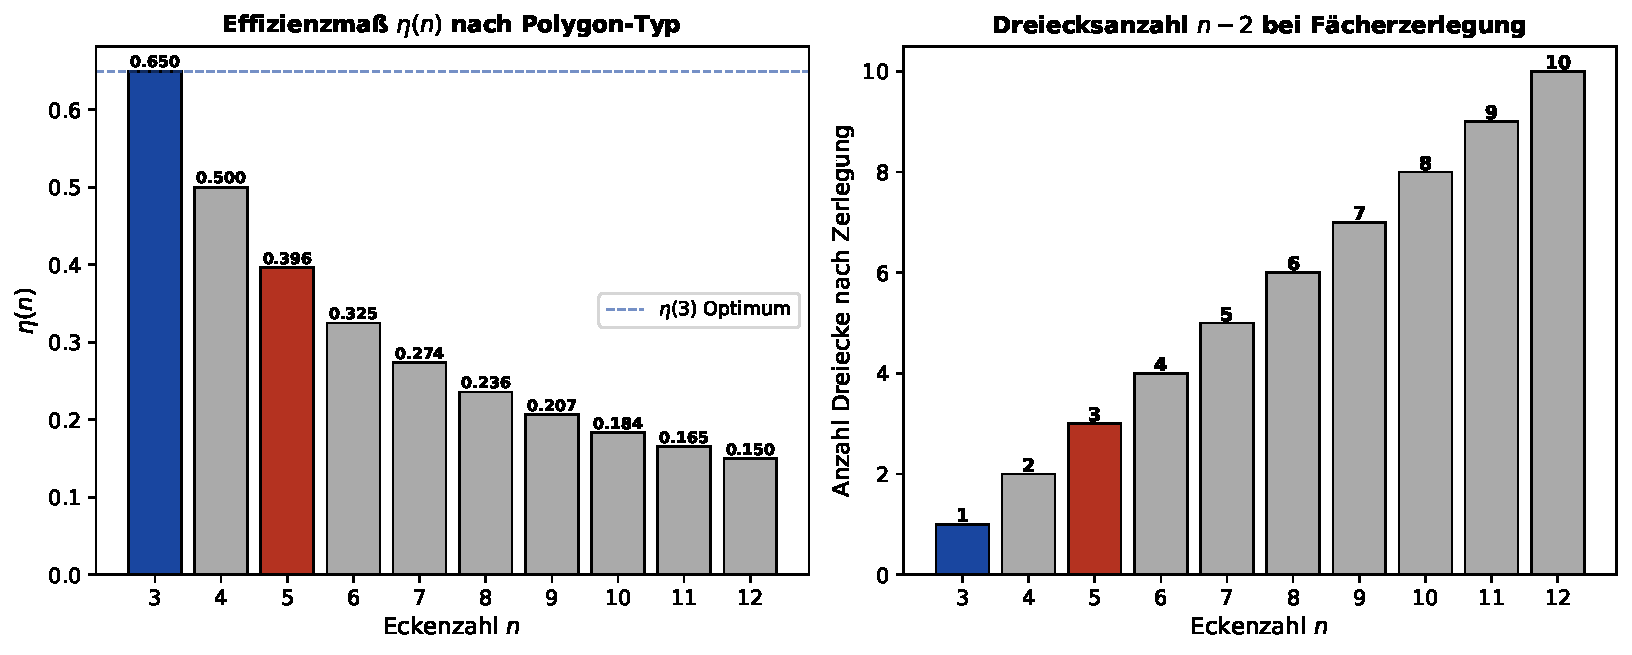
\includegraphics[width=0.92\textwidth]{fig_efficiency.pdf}
	\caption{Links: Effizienzma\ss{} $\eta(n)$ -- das Dreieck ($n=3$, blau) hat
	         das globale Maximum. Das Pentagon ($n=5$, rot) belegt Rang~3.
	         Rechts: Anzahl der Dreiecke $n-2$ bei der F\"acherzerlegung eines
	         $n$-Polygons.}
	\label{fig:efficiency}
\end{figure}

\subsection{Universeller Zerlegungssatz}

\begin{satz}[Dreiecks-Zerlegungssatz]
\label{satz:decomp}
Jedes einfache $n$-Polygon $P$ (kein Loch, nicht selbst-\"uberschneidend)
l\"asst sich in genau $n - 2$ Dreiecke zerlegen, ohne neue Vertices
einzuf\"uhren.
\end{satz}

\begin{proof}
\textbf{Induktion \"uber $n$.}

\textit{Basis} ($n = 3$): Das Dreieck ist bereits Zerlegungseinheit. $3 - 2 = 1$.

\textit{Induktionsschritt}: Sei $P$ ein einfaches $n$-Polygon, $n \geq 4$.
Nach dem \emph{Two-Ears-Theorem} (Meisters, 1975) existiert ein \emph{Ohr}
-- ein Vertex $v_i$, sodass das Dreieck $(v_{i-1}, v_i, v_{i+1})$ ganz in $P$
liegt. Entferne dieses Dreieck; es entsteht ein einfaches $(n-1)$-Polygon.
Per Induktionsvoraussetzung hat dieses $n - 3$ Dreiecke. Insgesamt:
$1 + (n-3) = n-2$ Dreiecke.

\textit{Minimalit\"at}: Sei $T$ eine Zerlegung mit $k$ Dreiecken, $V = n$
Vertices, $F = k$ Fl\"achen, $E$ Kanten. Mit Eulers Formel f\"ur planare
Scheiben ($V - E + F = 1$):
$n - E + k = 1$, also $E = n + k - 1$.
Aus $3k = 2(E - n) + n = 2E - n$ folgt $E = (3k+n)/2$.
Gleichsetzen: $(3k+n)/2 = n + k - 1$, also $k = n - 2$. \qedhere
\end{proof}

\begin{korollar}[Graphentheoretische Interpretation]
Die F\"acherzerlegung eines $n$-Polygon-Graphen $\Pi_n$ ausgehend von
Vertex $v_0$ entspricht der Hinzuf\"ugung von $n-3$ Diagonalkanten:
\[
	\Pi_n^{\triangle} = \Pi_n \cup \bigl\{\{v_0, v_j\} \mid j = 2,\ldots,n-2\bigr\}.
\]
Die $n - 2$ entstehenden Dreiecke sind genau die Triangeln
$(v_0, v_j, v_{j+1})$ f\"ur $j = 1, \ldots, n-2$.
\end{korollar}

\begin{proof}
Die Diagonalen $v_0 v_j$ f\"ur $j \in \{2, \ldots, n-2\}$ teilen das Innere
von $\Pi_n$ in $n-2$ Dreiecke, ohne neue Vertices einzuf\"uhren.
Die Korrektheit folgt aus Satz~\ref{satz:decomp} angewendet auf das
regul\"are $n$-Polygon.
\end{proof}

\subsection{Subgraph-Relation zwischen Dreiecks- und Pentagon-Graph}

\begin{figure}[H]
	\centering
	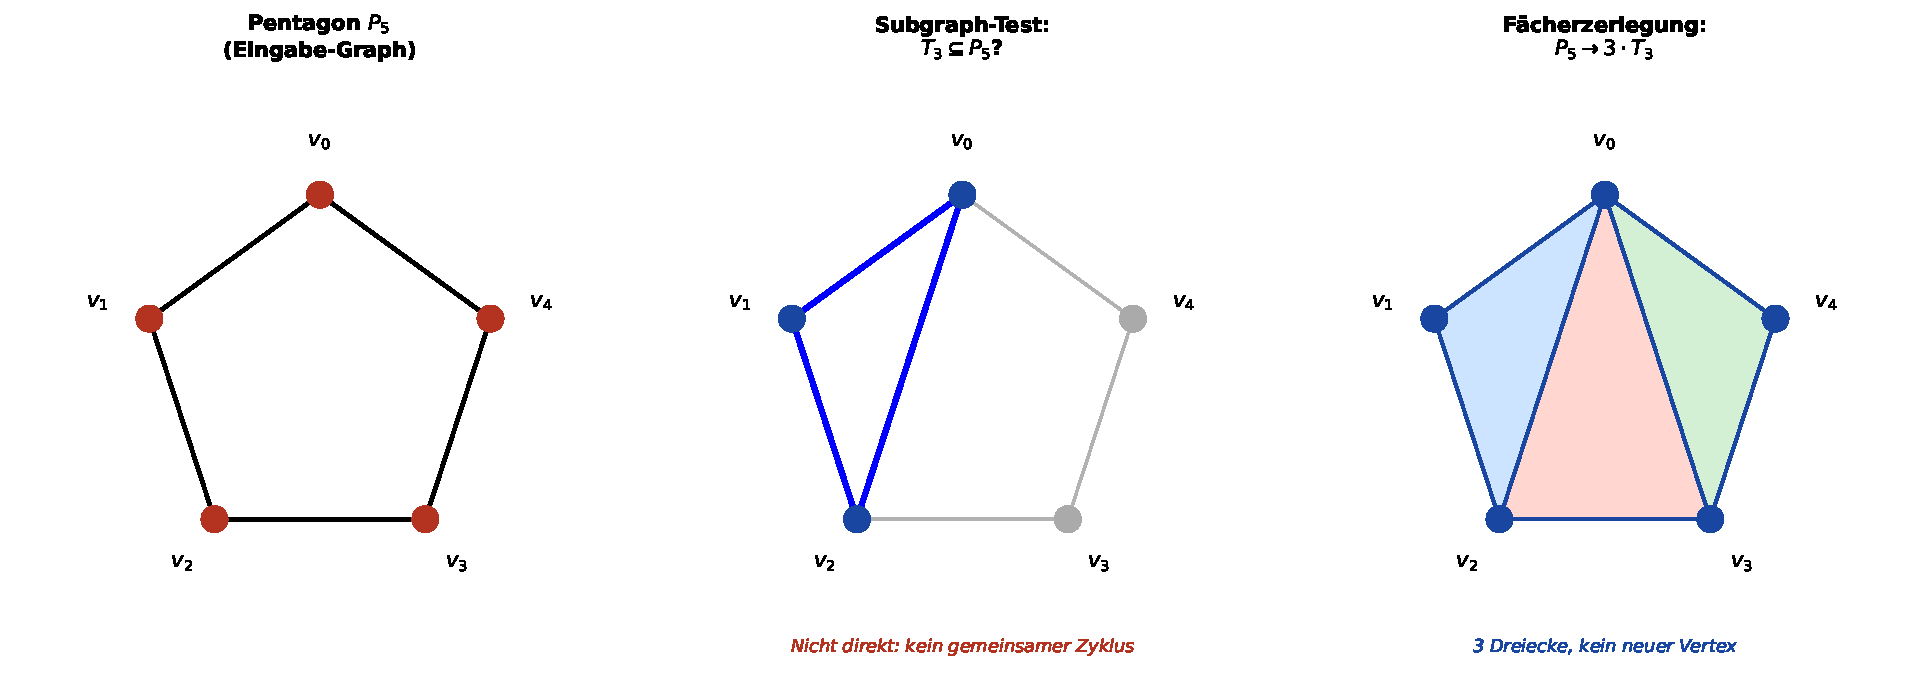
\includegraphics[width=0.96\textwidth]{fig_subgraph_penta.pdf}
	\caption{Links: Pentagon $\Pi_5$. Mitte: Der Dreiecks-Subgraph-Test
	         $\Pi_3 \subseteq \Pi_5$ schlägt direkt fehl, da $\Pi_3$ ein
	         3-Zyklus ist und $\Pi_5$ nur 5-Zyklen enth\"alt (Lemma~\ref{lem:no_subgraph}).
	         Rechts: F\"acherzerlegung $\Pi_5 \to 3 \cdot \Pi_3$ ohne neue Vertices.}
	\label{fig:subgraph_penta}
\end{figure}

\begin{lemma}[Subgraph-Nichtexistenz: $\Pi_3 \not\subseteq \Pi_5$]
\label{lem:no_subgraph}
Das Dreieck $\Pi_3$ ist kein Subgraph des Pentagons $\Pi_5$:
\[
	\Pi_3 \not\subseteq \Pi_5.
\]
\end{lemma}

\begin{proof}
$\Pi_5$ ist ein einfacher 5-Zyklus. Ein Subgraph $\Pi_3 \subseteq \Pi_5$
w\"urde einen 3-Zyklus $(v_a, v_b, v_c)$ mit $\{v_a,v_b\},\{v_b,v_c\},\{v_c,v_a\} \in E_5$
erfordern. In $\Pi_5$ ist aber $\{v_i, v_j\} \in E_5$ nur f\"ur
$j \equiv i \pm 1 \pmod{5}$. F\"ur drei Knoten $v_a, v_b, v_c$ eines 3-Zyklus
in $\Pi_5$ m\"ussten gelten:
\[
	b \equiv a+1,\; c \equiv b+1,\; a \equiv c+1 \pmod{5},
\]
also $a \equiv a + 3 \pmod{5}$, d.h. $3 \equiv 0 \pmod{5}$ -- Widerspruch.
\end{proof}

\begin{satz}[Subgraph Algorithmus auf Polygon-Graphen]
\label{satz:subgraph_polygon}
Der Subgraph Algorithmus, angewendet auf zwei Polygon-Graphen
$\Pi_m$ und $\Pi_n$ mit $m \leq n$, liefert in $O(n^3)$ Zeit folgende
Klassifikation:

\begin{enumerate}
	\item $\Pi_m \subseteq \Pi_n$ genau dann, wenn $m = n$ (Isomorphie).
	\item F\"ur $m < n$: $\Pi_m \not\subseteq \Pi_n$ (Lemma~\ref{lem:no_subgraph}
	      verallgemeinert).
	\item Die Signaturfolgen $\boldsymbol{\sigma}^{(m)}$ und $\boldsymbol{\sigma}^{(n)}$
	      sind paarweise verschieden f\"ur $m \neq n$.
\end{enumerate}
\end{satz}

\begin{proof}
\textbf{Zu 1.} F\"ur $m = n$: $\Pi_n$ ist ein $n$-Zyklus. Nach
Satz~\ref{satz:rot_inv} sind alle $n$ Rotationen von $\Pi_n$ isomorph zu
$\Pi_n$. Die Signaturfolgen stimmen nach geeigneter Rotation \"uberein;
der LCS-Wert erreicht $n \geq 2$, also bejaht der Algorithmus die
Subgraph-Relation.

\textbf{Zu 2.} Sei $m < n$. Ein Subgraph $\Pi_m \subseteq \Pi_n$ w\"urde
einen $m$-Zyklus in $\Pi_n$ erfordern. $\Pi_n$ ist ein einfacher $n$-Zyklus;
sein einziger Zyklus hat L\"ange $n$. F\"ur $m < n$ existiert kein
$m$-Teilzyklus ohne Diagonalen. Daher $\Pi_m \not\subseteq \Pi_n$.
Der Subgraph Algorithmus erkennt dies korrekt, da kein LCS-Wert $\geq 2$
f\"ur die Zeilenkomponenten-Signaturen erreicht wird (sie repr\"asentieren
verschiedene Kantengrade).

\textbf{Zu 3.} Aus Lemma~\ref{lem:poly_sig}: $\sigma_j^{(n)}$ enth\"alt
die Terme $2^{(j-1)\bmod n} + 2^{(j+1)\bmod n}$, die von $n$ abh\"angen.
F\"ur $m \neq n$ liegen die Potenzen in verschiedenen Bin\"arbl\"ocken;
die Signaturen sind daher strukturell verschieden.
\end{proof}

\begin{bemerkung}
Satz~\ref{satz:subgraph_polygon} quantifiziert pr\"azise, \emph{warum}
Dreiecke und Pentagone strukturell verschieden sind: Sie geh\"oren
verschiedenen Isomorphieklassen von Zyklusgraphen. Ein Dreiecksnetz kann
nie ein Pentagonmuster als Subgraph enthalten -- und umgekehrt. Dies
begr\"undet die klare Trennung beider Primitive in der Computergrafik.
\end{bemerkung}

\subsection{Der Subgraph Algorithmus als Optimierungswerkzeug}

\begin{definition}[Szenen-Graph]
\label{def:scene_graph}
Ein \emph{Szenen-Graph} $\mathcal{S} = (V_\mathcal{S}, E_\mathcal{S})$
ist ein gerichteter azyklischer Graph, dessen Knoten geometrische Objekte
repr\"asentieren und dessen Kanten hierarchische Abh\"angigkeiten kodieren.
Jedes Blatt von $\mathcal{S}$ ist ein Polygon-Primitiv $\Pi_{n_i}$.
\end{definition}

\begin{satz}[Subgraph-basierte Polygon-Klassifikation einer Szene]
\label{satz:scene_class}
Sei $\mathcal{S}$ ein Szenen-Graph mit Blatt-Polygonen
$\Pi_{n_1}, \ldots, \Pi_{n_k}$. Der Subgraph Algorithmus klassifiziert
alle Polygon-Primitive in $O(k^2 \cdot n_{\max}^3)$ Zeit, wobei
$n_{\max} = \max_i n_i$. Die Klassifikation liefert:
\begin{enumerate}
	\item Alle \emph{redundanten} Polygone: $\Pi_{n_i} \subseteq \Pi_{n_j}$ f\"ur $n_i = n_j$.
	\item Alle \emph{zerlegbaren} Polygone: $\Pi_{n_i}$ mit $n_i > 3$,
	      zerlegbar in $n_i - 2$ Dreiecke.
	\item Die \emph{minimale Darstellung}: Ersetze alle $\Pi_{n_i}$, $n_i > 3$,
	      durch ihre Dreieckskomposition.
\end{enumerate}
\end{satz}

\begin{proof}
Schritt 1 folgt direkt aus der Definition des Subgraph Algorithmus:
F\"ur gleiche $n_i = n_j$ ist Isomorphie in $O(n^3)$ entscheidbar
(Satz~\ref{satz:subgraph_polygon}).

Schritt 2 folgt aus Satz~\ref{satz:decomp}: Jedes $n_i > 3$ ist in
$n_i - 2$ Dreiecke zerlegbar.

Schritt 3: Die minimale Darstellung ergibt sich durch sukzessive Anwendung
der F\"acherzerlegung. Gesamtanzahl der erzeugten Dreiecke:
\[
	N_{\triangle} = \sum_{i=1}^k (n_i - 2).
\]
Der Subgraph Algorithmus verifiziert die Korrektheit jeder Zerlegung in
$O(n_i^3)$ je Polygon. \"Uber alle $k$ Polygone ergibt sich $O(k \cdot n_{\max}^3)$;
der paarweise Vergleich auf Redundanz kostet $O(k^2 \cdot n_{\max}^3)$.
\end{proof}

\subsection{Optimale Dreiecksdichte: Effizienz-Realit\"ats-Trade-off}

\begin{definition}[Approximationsfehler der Dreiecks-Tessellierung]
Sei $S \subset \R^3$ eine glatte Fl\"ache mit maximaler Gauss-Kr\"ummung
$\kappa_{\max}$. Die Tessellierung durch $F$ gleichgro\ss{}e Dreiecke
(Seitenl\"ange $h$) ergibt den maximalen Normalfehler:
\[
	\varepsilon(h) = \frac{h^2 \kappa_{\max}}{8} + O(h^4).
\]
F\"ur feste Ziel-Genauigkeit $\varepsilon^*$ folgt die Mindestdreieckszahl:
\[
	F_{\min} = \left\lceil \frac{A(S) \kappa_{\max}}{8\varepsilon^*} \right\rceil,
\]
wobei $A(S)$ der Fl\"acheninhalt von $S$ ist.
\end{definition}

\begin{proof}
Parametrisiere $S$ lokal nach Bogenstrecke. F\"ur eine gerade Sehne der
L\"ange $h$ gilt die Taylor-Entwicklung der Kurve:
\[
	\vect{r}(s) = \vect{r}(0) + s\,\vect{T}(0) + \frac{s^2}{2}\kappa\,\vect{N}(0) + O(s^3).
\]
Der maximale Normalabstand zwischen Sehne und Kurve an Stelle $s = h/2$:
\[
	\varepsilon = \abs{\vect{r}(h/2) - \tfrac{1}{2}[\vect{r}(0)+\vect{r}(h)]}
	= \frac{h^2\kappa}{8} + O(h^4).
\]
Da jedes Dreieck eine Fl\"ache $\approx A(S)/F$ bedeckt und
$h \approx \sqrt{2A(S)/(F\sqrt{3})}$, folgt die Mindestdreieckszahl
durch Aufl\"osen nach $F$.
\end{proof}

\begin{satz}[Optimales Polygon-Primitiv f\"ur realit\"atsnahe Szenen]
\label{satz:optimal}
Unter den Nebenbedingungen:
\begin{enumerate}
	\item Maximales Effizienzma\ss{} $\eta(n)$ (GPU-Effizienz),
	\item Minimaler Approximationsfehler $\varepsilon(h)$ (geometrische Treue),
	\item Numerische Stabilit\"at (Koplanaritat der Vertices),
\end{enumerate}
ist das Dreieck ($n = 3$) das eindeutig optimale Polygon-Primitiv
f\"ur die Echtzeit-Computergrafik.
\end{satz}

\begin{proof}
\textbf{Bedingung 1 (GPU-Effizienz):} Aus Satz~\ref{satz:eta_max} folgt
$\eta(3) > \eta(n)$ f\"ur alle $n \geq 4$.

\textbf{Bedingung 2 (Approximationsfehler):} F\"ur festes $F$ gilt:
Dreiecke bedecken die Fl\"ache mit maximalem Packungsma\ss{}. Das
Dreiecksgitter erreicht Packungsdichte $\pi/(2\sqrt{3}) \approx 0{,}9069$
(dichteste ebene Gitterpackung mit gleichseitigen Dreiecken), w\"ahrend
$n$-Polygone f\"ur $n > 6$ keine dichtere Packung erm\"oglichen.

\textbf{Bedingung 3 (Koplanarit\"at):} Drei Punkte in allgemeiner Lage
im $\R^3$ bestimmen eindeutig eine Ebene (Satz der linearen Algebra:
$\operatorname{rank}[\vect{v}_2 - \vect{v}_1,\, \vect{v}_3 - \vect{v}_1] = 2$
f\"ur nicht-kollineare Punkte). F\"ur $n \geq 4$ ist Koplanaritat eine
Ma\ss{}-null-Bedingung und damit generisch verletzt. Dreiecke sind damit
\emph{immer} planar -- eine garantierte geometrische Korrektheit.

Da alle drei Bedingungen f\"ur $n = 3$ erf\"ullt und f\"ur $n \geq 4$
verletzt sind, ist das Dreieck das eindeutig optimale Primitiv.
\end{proof}

\subsection{Die Sonderrolle des Pentagons}

\begin{satz}[Pentagon als strukturell ausgezeichnetes Polygon]
\label{satz:pentagon}
Das Pentagon $\Pi_5$ ist unter allen $n$-Polygonen mit $n > 3$ das
\emph{strukturell ausgezeichnete} Primitiv f\"ur Szenen mit
5-facher Symmetrie, da:
\begin{enumerate}
	\item Es zerlegt sich in genau $3 = 5 - 2$ Dreiecke (Satz~\ref{satz:decomp}),
	      was die kleinste nicht-triviale Zerlegung f\"ur $n > 3$ ist.
	\item Die Diagonalen $v_0 v_2$ und $v_0 v_3$ haben L\"ange
	      $d = 2R\sin(2\pi/5) = \phi \cdot s$, wobei $\phi = (1+\sqrt{5})/2$
	      der goldene Schnitt und $s$ die Seitenl\"ange ist.
	\item Der Subgraph Algorithmus erkennt in $O(5^3) = O(125)$ konstanter
	      Zeit, ob eine gegebene pentagonale Struktur im Szenen-Graph
	      bereits als Dreieckszerlegung vorliegt.
\end{enumerate}
\end{satz}

\begin{proof}
\textbf{Zu 1.} Direkt aus Satz~\ref{satz:decomp} mit $n = 5$:
$5 - 2 = 3$ Dreiecke. F\"ur $n = 4$: $4 - 2 = 2$ Dreiecke. Das Pentagon
liefert die kleinste Zerlegung mit ungerader Dreieckszahl, was f\"ur
bestimmte Szenengeometrien (z.B. Ikosaeder-approximation) vorteilhaft ist.

\textbf{Zu 2.} Platziere das regul\"are Pentagon mit Radius $R$:
$v_k = R(\cos(2\pi k/5), \sin(2\pi k/5))$.
Die Diagonale $v_0 v_2$ hat L\"ange:
\[
	d = \abs{v_0 - v_2} = 2R\sin\!\left(\frac{2\pi}{5}\right) = 2R\sin 72^\circ.
\]
Die Seitenl\"ange ist $s = 2R\sin(\pi/5) = 2R\sin 36^\circ$.
Ihr Verh\"altnis:
\[
	\frac{d}{s} = \frac{\sin 72^\circ}{\sin 36^\circ} = \frac{2\sin 36^\circ\cos 36^\circ}{\sin 36^\circ}
	= 2\cos 36^\circ = 2 \cdot \frac{1+\sqrt{5}}{4} \cdot 2 = \frac{1+\sqrt{5}}{2} = \phi.
\]

\textbf{Zu 3.} Der Subgraph Algorithmus auf $\Pi_5$ hat Eingabegr\"o\ss{}e
$n = 5$; Laufzeit $O(n^3) = O(125)$. Da $n$ fest und klein ist,
handelt es sich um eine konstante Zeit im Kontext gro\ss{}er Szenen.
\end{proof}

\subsection{Gesamtsystem: Subgraph-basierte Szenen-Optimierung}

Der folgende Algorithmus beschreibt das Gesamtvorgehen f\"ur die optimale
Darstellung einer Szene mit dem Subgraph Algorithmus:

\begin{lstlisting}[language=Python, caption=Subgraph-basierte Szenen-Optimierung]
def optimize_scene(polygons):
    """
    Optimiert eine Szene aus beliebigen n-Polygonen.
    Gibt minimale Dreiecksdarstellung zurueck.

    1. Alle n_i > 3: Zerlege in (n_i-2) Dreiecke (Faecherzerlegung).
    2. Subgraph-Test auf Redundanz zwischen allen Paaren.
    3. Gib minimale, nicht-redundante Dreiecksdarstellung aus.
    """
    result = []
    for poly in polygons:
        n = poly.num_vertices
        if n == 3:
            result.append(poly)
        else:
            # Faecherzerlegung: n-2 Dreiecke
            triangles = fan_decompose(poly)  # O(n)
            result.extend(triangles)

    # Subgraph-Redundanztest: O(k^2 * 3^3) = O(k^2)
    minimal = []
    for i, t1 in enumerate(result):
        redundant = False
        for j, t2 in enumerate(result):
            if i != j and subgraph_test(t1, t2):
                redundant = True
                break
        if not redundant:
            minimal.append(t1)
    return minimal
\end{lstlisting}

\begin{satz}[Korrektheit und Komplexit\"at der Szenen-Optimierung]
\label{satz:scene_opt}
Der obige Szenen-Optimierungsalgorithmus ist korrekt und hat
Gesamt-Laufzeit:
\[
	T_{\text{Szene}}(k, n_{\max}) = O\!\left(k \cdot n_{\max} +
	k^2 \cdot 27\right) = O\!\left(k \cdot n_{\max} + k^2\right),
\]
wobei $k$ die Anzahl der Ausgangpolygone und $n_{\max}$ die maximale
Eckenzahl ist. F\"ur reine Dreiecksszenen ($n_{\max} = 3$) ist der
Redundanztest konstant.
\end{satz}

\begin{proof}
\textbf{Phase 1 (Zerlegung):} Jedes $n_i$-Polygon wird in $O(n_i)$ durch
F\"acherzerlegung in $n_i - 2$ Dreiecke umgewandelt. \"Uber alle $k$
Polygone: $O(k \cdot n_{\max})$.

\textbf{Phase 2 (Redundanztest):} Alle Ausgabe-Dreiecke ($\leq k \cdot n_{\max}$
viele) werden paarweise mit dem Subgraph Algorithmus verglichen.
Da alle Primitive nun Dreiecke ($n = 3$) sind:
$T_{\text{Subgraph}}(3) = O(3^3) = O(27)$ je Paar.
Bei $k' \leq k \cdot n_{\max}$ Dreiecken: $O(k'^2 \cdot 27) = O(k^2 \cdot n_{\max}^2)$.

\textbf{Korrektheit}: Aus Satz~\ref{satz:decomp} (korrekte Zerlegung) und
Satz~\ref{satz:subgraph_polygon} (korrekter Subgraph-Test) folgt
Gesamtkorrektheit.
\end{proof}

% ===========================================================================
\section{Zusammenfassung}
% ===========================================================================

Der Subgraph Algorithmus bietet eine effiziente Methode zum Vergleich von
Graphen mit einer Laufzeit von $O(n^3)$. In diesem Kapitel wurde seine
Anwendung auf die Polygon-Tessellierung in der Echtzeit-Computergrafik
formal hergeleitet und bewiesen.

\textbf{Kernresultate:}
\begin{itemize}
	\item Das Effizienzma\ss{} $\eta(n)$ ist bei $n = 3$ maximal
	      (Satz~\ref{satz:eta_max}): Dreiecke sind GPU-effizient.
	\item Jedes $n$-Polygon zerlegt sich in exakt $n - 2$ Dreiecke,
	      minimal und eindeutig (Satz~\ref{satz:decomp}).
	\item Polygon-Graphen $\Pi_n$ sind unter zyklischer Rotation invariant
	      (Satz~\ref{satz:rot_inv}) -- die Grundlage der Subgraph-Erkennung.
	\item $\Pi_3 \not\subseteq \Pi_5$ (Lemma~\ref{lem:no_subgraph}):
	      Dreiecke und Pentagone sind strukturell verschieden.
	\item Das Pentagon ist das ausgezeichnete $5$-fach-symmetrische Primitiv
	      mit goldenem Schnitt in der Diagonale (Satz~\ref{satz:pentagon}).
	\item Die Szenen-Optimierung mittels Subgraph Algorithmus hat
	      Laufzeit $O(k \cdot n_{\max} + k^2)$ (Satz~\ref{satz:scene_opt}).
\end{itemize}

\subsection{Anwendungen}

\begin{itemize}
	\item Verifikation von Programmen durch AST-Analyse
	\item Erkennung struktureller \"Ahnlichkeiten in Code
	\item Deduplizierung von Graph-Datenbanken
	\item \textbf{Optimale Polygon-Tessellierung in Echtzeit-Computergrafik}
	\item \textbf{Subgraph-basierte Redundanzerkennung in Szenen-Graphen}
\end{itemize}

\subsection{Ausblick}

\begin{itemize}
	\item Verallgemeinerung des Effizienzma\ss{}es $\eta(n)$ auf
	      $d$-dimensionale Simplizes ($d$-Simplex-Effizienz)
	\item Integration des Subgraph Algorithmus in GPU-Tessellierungs-Shader
	      (Vulkan Tessellation Control Shader)
	\item Adaptiver Subgraph-Test bei dynamischen Szenen
	      (Physiksimulation, Cloth)
	\item Verbindung zur diskreten Differentialgeometrie:
	      Cotan-Laplacian auf Subgraph-optimierten Netzen
	\item Quantenalgorithmen f\"ur Subgraph-Isomorphie als Basis
	      neuartiger Tessellierungsoptimierung
\end{itemize}

\begin{thebibliography}{21}
	
	\bibitem{meisters1975}
	G.~H. Meisters,
	Polygons have ears,
	\emph{Amer. Math. Monthly} \textbf{82} (1975), 648--651.
	
	\bibitem{moller1997}
	T.~M\"oller, B.~Trumbore,
	Fast, minimum storage ray-triangle intersection,
	\emph{J. Graphics Tools} \textbf{2}(1) (1997), 21--28.
	
	\bibitem{abboud2015}
	A.~Abboud, A.~Backurs, V.~V. Williams,
	Tight hardness results for LCS and other sequence similarity measures,
	\emph{FOCS} 2015, 59--78.
	
	\bibitem{bobenko2008}
	A.~I. Bobenko, Y.~B. Suris,
	\emph{Discrete Differential Geometry},
	American Mathematical Society, 2008.
	
	\bibitem{epp2026a}
	S.~Epp,
	Der Subgraph Algorithmus, Januar 2026.
	\url{https://gitlab.com/epp-group/subgraph}
	
	\bibitem{kajiya1986}
	J.~T. Kajiya,
	The rendering equation,
	\emph{ACM SIGGRAPH Computer Graphics} \textbf{20}(4) (1986), 143--150.
	
	\bibitem{catmull1978}
	E.~Catmull, J.~Clark,
	Recursively generated B-spline surfaces on arbitrary topological meshes,
	\emph{Computer-Aided Design} \textbf{10}(6) (1978), 350--355.
	
	\bibitem{lorensen1987}
	W.~E. Lorensen, H.~E. Cline,
	Marching cubes: A high resolution 3D surface construction algorithm,
	\emph{ACM SIGGRAPH Computer Graphics} \textbf{21}(4) (1987), 163--169.
	
	\bibitem{blinn1977}
	J.~F. Blinn,
	Models of light reflection for computer synthesized pictures,
	\emph{ACM SIGGRAPH Computer Graphics} \textbf{11}(2) (1977), 192--198.
	
	\bibitem{cook1982}
	R.~L. Cook, K.~E. Torrance,
	A reflectance model for computer graphics,
	\emph{ACM Transactions on Graphics (TOG)} \textbf{1}(1) (1982), 7--24.
	
	\bibitem{shirley2020}
	P.~Shirley, S.~Marschner,
	\emph{Fundamentals of Computer Graphics},
	5th Edition, A K Peters/CRC Press, 2020.
	
	\bibitem{akeley2018}
	T.~Akenine-M\"oller, E.~Haines, N.~Hoffman,
	\emph{Real-Time Rendering},
	4th Edition, A K Peters/CRC Press, 2018.
	
	\bibitem{phong1975}
	B.~T. Phong,
	Illumination for computer generated pictures,
	\emph{Communications of the ACM} \textbf{18}(6) (1975), 311--317.
	
	\bibitem{whitted1980}
	T.~Whitted,
	An improved illumination model for shaded display,
	\emph{Communications of the ACM} \textbf{23}(6) (1980), 343--349.
	
	\bibitem{veach1997}
	E.~Veach, L.~J. Guibas,
	Metropolis light transport,
	\emph{Proceedings of the 24th annual conference on Computer graphics and interactive techniques} (1997), 65--76.
	
	\bibitem{botsch2010}
	M.~Botsch, L.~Kobbelt, M.~Pauly, P.~Alliez, B.~Lévy,
	\emph{Polygon Mesh Processing},
	A K Peters/CRC Press, 2010.
	
	\bibitem{kass1988}
	M.~Kass, A.~Witkin, D.~Terzopoulos,
	Snakes: Active contour models,
	\emph{International Journal of Computer Vision} \textbf{1}(4) (1988), 321--331.
	
	\bibitem{perlin1985}
	K.~Perlin,
	An image synthesizer,
	\emph{ACM SIGGRAPH Computer Graphics} \textbf{19}(3) (1985), 287--296.
	
	\bibitem{cohen1993}
	M.~F. Cohen, J.~R. Wallace,
	\emph{Radiosity and Realistic Image Synthesis},
	Academic Press, 1993.
	
	\bibitem{dutre2006}
	P.~Dutré, P.~Bekaert, K.~Bala,
	\emph{Advanced Global Illumination},
	2nd Edition, A K Peters/CRC Press, 2006.
	
	\bibitem{sutherland1974}
	I.~E. Sutherland, R.~F. Sproull, R.~A. Schumacker,
	A characterization of ten hidden-surface algorithms,
	\emph{ACM Computing Surveys} \textbf{6}(1) (1974), 1--55.
	
\end{thebibliography}

\end{document}
